\begin{figure*}[t]
    \centering
    % TODO: change the image base size in order to remove the skewness effect
    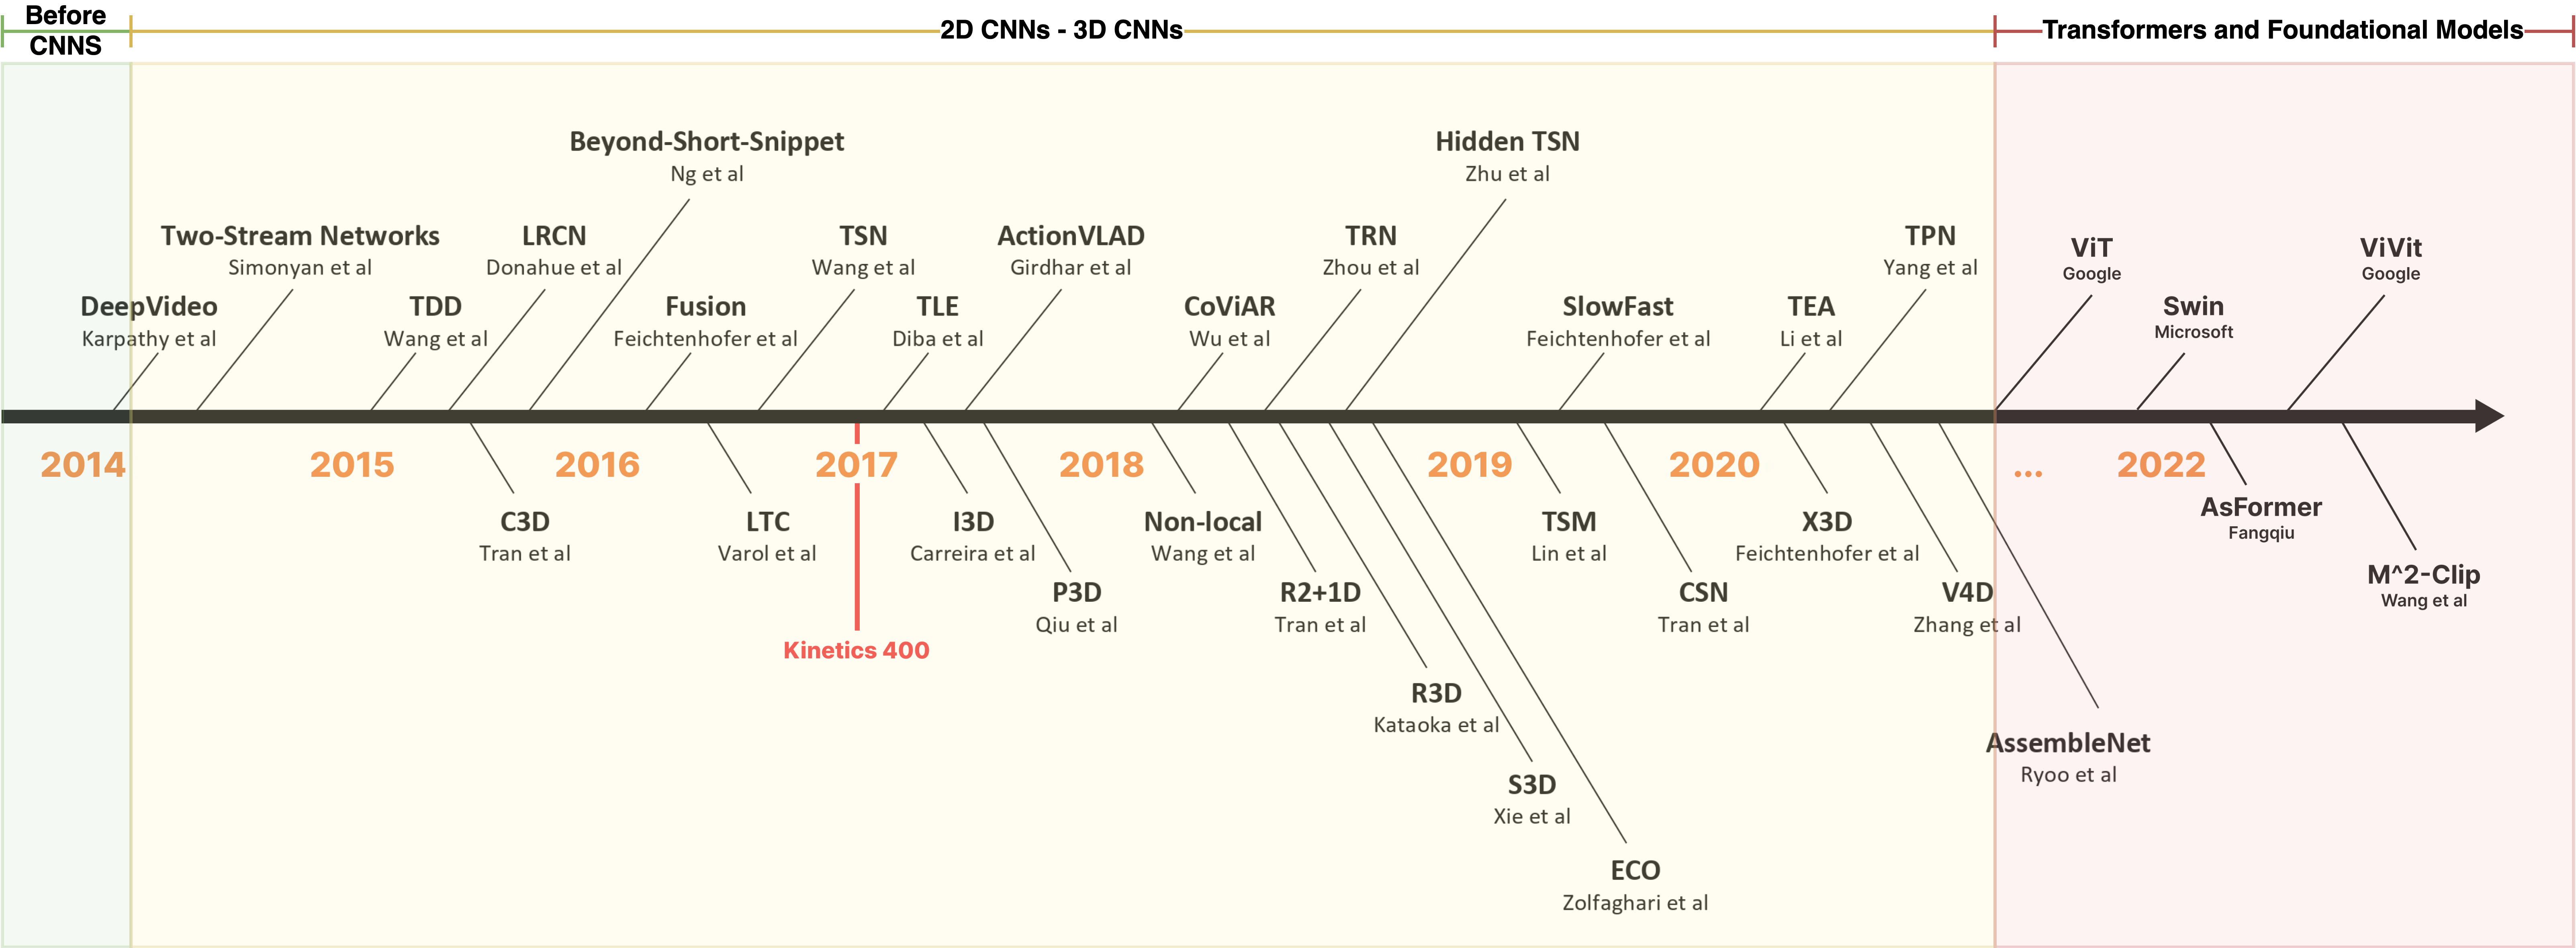
\includegraphics[width=\textwidth, height=0.25\textwidth]{../../assets/figures/extended-video-timeline-v3.png}
    \caption{A timeline overview of the evolution of video analysis models.}
    \label{fig:your-label}
\end{figure*}

\section{Related Work}

\todo[inline]{We could also have a cahrt showing the evolution of accuracy and number of papers on the field with time, and on the time axis we put markers for different events such as the release of popular datasets, improvements in compute power, etc.}

In this section we'll explore some popular temporal action segmentation methods.

Compared to image and text data, video data is very limited in the available datasets (although we have cited many in the previous popular-datasets section). In addition to that vidoe networks are very computationally costy, all this can be the reason that video related networks and the field is kind of left a little bit behind compared to other format of data.

But throughout the years an improvement have been seen with the rise of computational power. The very first methods relaied on hand feature extraction and specific pixels, then the next generation of networks started using optical flow, later 2D CNNs started to be used for feature extraction from video as they become popular and their success have been seen for videos. And then 3D Temporal CNNs with some optimizations have been started to be used with the raize of computational power and more importantly the 
availability of larger datasets such as Kinetics from google that is based on videos and other video datasets such as the something something, howto100m, etc. Lately transformers have been used too for that as more data is becoming available to support the transformers demand in data.

It is important to know that all the methods that'll be cited be low are rather demanding in temr of data and thus won't be applied directly on our dataset.

\todo[inline]{RePhrase: Talk about the different approaches and techniques. Talk about their evolution just like it is done in \textbf{ViViT: A Video Vision Transformer} paper. (First started by using hand collected features, 2D CNNs, 3D with optical flow, full 3d, transformers as the datasets started to grow, etc.)}

\todo[inline]{Do an illustration of that, like a small one for the evolution of networks and their architecture}

Video data presents a challenging problem due to its vast and diverse distribution, causing models to drift more rapidly compared to other data types. As a result, handling video data often requires significantly larger datasets. Even pre-trained models struggle to generalize well beyond their original training sets, making this an active area of ongoing research.

First of all we have to say that Temporal Action Segmentation can be expressed and viewed in different ways, for each one we'll cite some methods.

\textbf{Video Classification}

\textbf{Temporal Action Detection / Localization}

\textbf{Third Perspective}

Note that to view the problem in a video classification problem as it is the most popular perspective / field among the cited one \& thus there is more material on it to study it and more available pre-trained networks which is important considering the constraints that have been listed and that'll be later too during the 6-our-approach section.

\todo[inline]{Talk about the importance of TAS and its applications.}